\section{Set Notation}

\subsection{Introduction}

In this activity, we will solve problems similar to the one in Figure \ref{fig:2.1.1}.

\begin{figure}[h]
	\centering
	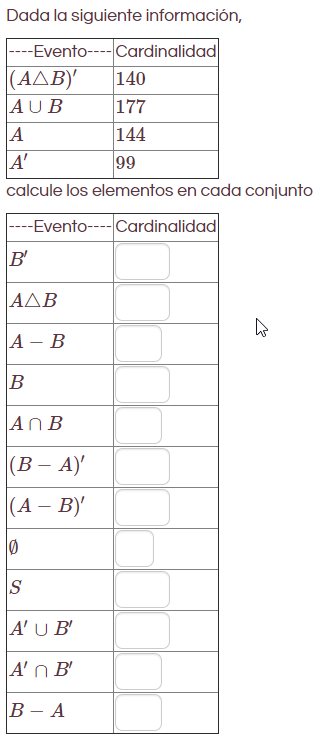
\includegraphics[width=0.7\linewidth]{images/2020-08-15-19_49_02.png}
	\caption{Counting problem}
	\label{fig:2.1.1}
\end{figure}

We will approach the problem using the following plan:
\begin{enumerate}
	\item Define a partition on a set.
	\item Establish a standard partition to describe operations between two sets. 
	\item Describe set operations using this partition.
	\item Formulate and solve the problem in terms of this partition. 
\end{enumerate}

As prerequisites, the following concepts are required:
\begin{enumerate}
	\item Sets and subsets.
	\item Set operations.
	\item Solution of systems of linear equations. 
\end{enumerate}

For clarity, we recall some definitions for subsets $ A,B \subset S $:
\begin{itemize}
	\item Union
	\[ A\cup B = \sett{x\in S}{x \in A \texttt{ or } x \in B} \]
	\item Intersection
	\[ A\cap B = \sett{x \in S}{x\in A \texttt{ and } x\in B}\]
	\item Set Difference (Relative Complement)  
	\[ A\backslash B = \sett{x\in S}{x\in A \texttt{ and } x\not \in B}\]
	Sometimes set difference is also denoted by $ A-B $. 
	\item Complement
	\[ A' = \sett{x\in S}{x\not \in A} \]
	The complement is sometimes also denoted by $ A^{c} $ or $ \bar{A} $. Equivalently, it can be written as $ S\backslash A.$
	\item Symmetric Difference
	\[ A\triangle B = \sett{x \in S}{x\in A \texttt{ or } x\in B \texttt{ but } x\not \in A\cap B}\]. 
\end{itemize}



\subsection{Partitions}

Consider a set $ S $. A (finite) partition is a collection $ \set{P_i \subset S}_{i=0}^{N}, N \in \N $ of subsets of $ S $ satisfying:
\begin{enumerate}
	\item $ P_i \cap P_j =\emptyset $ whenever $ i\neq j $;
	\item $ \bigcup_{i=0}^{N} P_i = S $. 
\end{enumerate}

In other words, they are mutually disjoint subsets that, when combined together, form the entire set $ S $. The reader can think of them as pieces of a jigsaw puzzle.

\begin{figure}
	\centering
	
\includegraphics[width=0.7\linewidth]{images/puzzle-5294291_1280}
	\caption[Jigsaw puzzle]{Jigsaw puzzles are examples of partitions.}
	\label{fig:2.1.2}
\end{figure}

Consider two sets $ A,B \subset S$. The corresponding Venn diagram is shown in Figure \ref{fig:2.1.3}.

\begin{figure}
	\centering
	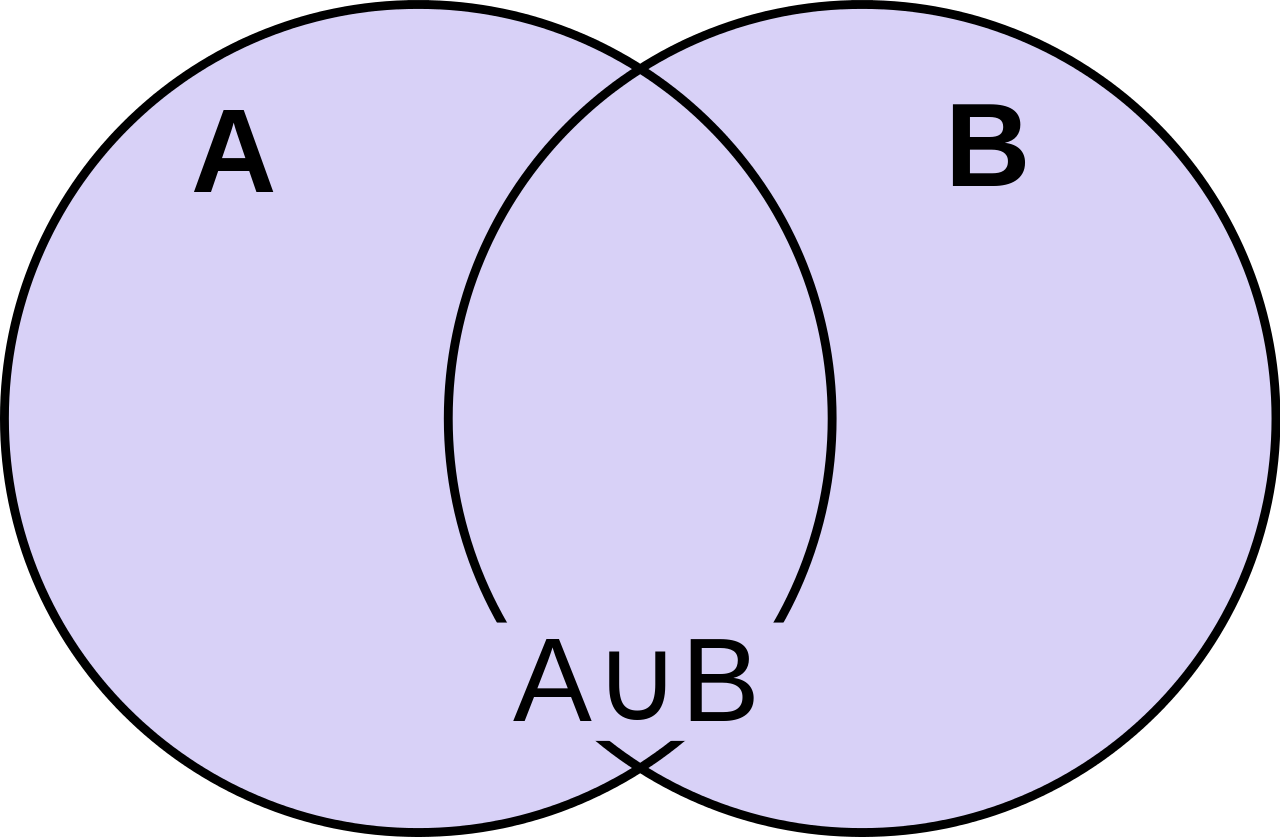
\includegraphics[width=0.7\linewidth]{images/1280px-Venn_diagram_for_A_union_B.svg}
	\caption{Venn diagram for two sets}
	\label{fig:2.1.3}
\end{figure}

We can define a partition $ \particion(A,B) $ of $ S $ with the following elements:
\begin{itemize}
	\item $ A\cap B $
	\item $ A\backslash B = A \cap B'$
	\item $ B\backslash A = B \cap A'$
	\item $ \left(A\cup B\right)' = A'\cap B' $
\end{itemize}

To make the notation more concise, we define the following indicator mappings:
\begin{align}
	\delta_C(x) = \begin{cases}
		1 & x \in C \\
		0 & x \not \in C
	\end{cases}
\end{align}
where $ 1 $ denotes \texttt{true}, while $ 0 $ denotes \texttt{false}, and
\begin{align}
	E_{(i,j)}=\sett{x\in S}{\delta_{A}(x)=i\wedge\delta_{B}(x)=j}
\end{align}
So that:
\begin{itemize}
	\item $ A' \cap B' = E_{(0,0)}$
	\item $ A'  \cap B = E_{(0,1)}$
	\item $ A \cap B'  = E_{(1,0)}$
	\item $ A  \cap B  = E_{(1,1)}$
\end{itemize}

To make the notation even simpler, we identify the pair $ (i,j) $ with its corresponding binary number $ [ij]_{2} $ converted to base 10. Thus:
\begin{itemize}
	\item $ A' \cap B' = E_{0}$
	\item $ A'  \cap B = E_{1}$
	\item $ A \cap B'  = E_{2}$
	\item $ A  \cap B  = E_{3}$
\end{itemize}

\subsection{Problem Formulation}

Since the elements of a partition are disjoint, we know that:
\begin{align}
	\#\left(E_i\cup E_j\right) = \#E_i+\#E_j
\end{align}
whenever $ i\neq j $.

To simplify the notation, we define $ x_i=\# E_i. $

The first equation given to us is:
\begin{align}
	\left(A \triangle B \right)'=140,
\end{align}
where 
\begin{align}
	A\triangle B = (A\backslash B)\cup(B\backslash A)
\end{align}
is the symmetric difference between $ A $ and $ B $. In other words, $ x\in A \triangle B $ if and only if $ x\in A $ or $ x \in B $ but not both.

Notice that then:
\begin{align}
	\label{eq:2.1.1}
	\left(A\triangle B\right)' = E_0 \cup E_3 &
	\Rightarrow
	x_0 + x_3 = 140.
\end{align}

Similarly, we arrive at the following conclusions:
\begin{align}
	\label{eq:2.1.2}
	A\cup B = E_1\cup E_2 \cup E_3 &
	\Rightarrow x_1+x_2+x_3=177 \\
	\label{eq:2.1.3}
	A = E_2 \cup E_3 &
	\Rightarrow x_2+x_3 = 144 \\
	\label{eq:2.1.4}
	A' = E_0 \cup E_1 &
	\Rightarrow x_0+x_1 =99
\end{align}

By solving the system of equations given by \eqref{eq:2.1.1}--\eqref{eq:2.1.4}, we obtain the solution:
\begin{align}
	x_0 &= 66 \\
	x_1 &= 33 \\
	x_2 &= 70 \\
	x_3 &= 74
\end{align}

\subsection{Problem Solution}

Below we present the derivation and conclusion for each of the questions in our problem. For example, we can describe the complement of $ B $ in terms of our partition and use our previous solutions:

\begin{align}
	\# B' 
	&= \#\left(E_1 \cup E_3\right)'\\
	&= \#\left(E_0 \cup E_2\right)\\
	&= x_0 + x_2 = 153
\end{align}

The rest of the solutions are found as follows:

\begin{align}
	\card{A\triangle B} = x_1+x_2 = 103  \\
	\card{A\backslash B} = x_2 = 70 \\
	\card{B} = x_1+x_3=107	\\
	\card{A \cap B} = x_3 = 74 \\
	\card{\left(B\backslash A\right)'} 
	= x_0+x_2+x_3 = 210 \\
	\card{\left(A\backslash B\right)'}
	= x_0+x_1+x_3 = 173 \\
	\card{\emptyset} = 0 \\
	\card{S} = x_0+x_1+x_2+x_3 = 243 \\
	\card{A' \cap B'} = x_0 = 66\\
	\card{B\backslash A} = x_1 = 33
\end{align}

This concludes our exercise.
